% Link color
% Set link colors throughout the document


\documentclass[12pt]{article}
%%%%%%%%%%%%%%%%%%%%%%%%%%%%%%%%%%%%%%%%%%%%%%%%%%%%%%%%%%%%%%%%%%%%%%%%%%%%%%%%%%%%%%%%%%%%%%%%%%%%%%%%%%%%%%%%%%%%%%%%%%%%%%%%%%%%%%%%%%%%%%%%%%%%%%%%%%%%%%%%%%%%%%%%%%%%%%%%%%%%%%%%%%%%%%%%%%%%%%%%%%%%%%%%%%%%%%%%%%%%%%%%%%%%%%%%%%%%%%%%%%%%%%%%%%%%
\usepackage{natbib}
\usepackage{mathptmx}
\usepackage[latin9]{inputenc}
\usepackage{geometry}
\usepackage{pdflscape}
\usepackage{color}
\usepackage{float}
\usepackage{amsmath}
\usepackage{setspace}
\usepackage{a4wide}
\usepackage{hyperref}
\usepackage{rotating}
\usepackage{graphicx}
\usepackage{threeparttable}
\usepackage{graphicx}
\usepackage{setspace}
\usepackage{lscape}
\usepackage{booktabs}
\usepackage{hyperref}
\usepackage{xr-hyper}

\setcounter{MaxMatrixCols}{10}
%TCIDATA{OutputFilter=LATEX.DLL}
%TCIDATA{Version=5.50.0.2960}
%TCIDATA{<META NAME="SaveForMode" CONTENT="1">}
%TCIDATA{BibliographyScheme=BibTeX}
%TCIDATA{LastRevised=Tuesday, December 19, 2017 14:55:35}
%TCIDATA{<META NAME="GraphicsSave" CONTENT="32">}
%TCIDATA{Language=American English}
%TCIDATA{CSTFile=article.cst}

\newcommand{\noop}[1]{}
\definecolor{linkcolour}{rgb}{0,0.2,0.6} 
\definecolor{airforceblue}{rgb}{0.36, 0.54, 0.66}
\definecolor{blue(pigment)}{rgb}{0.2, 0.2, 0.6}
\definecolor{coolblack}{rgb}{0.0, 0.18, 0.39}
\hypersetup{colorlinks,breaklinks,urlcolor=linkcolour,linkcolor=linkcolour,citecolor={coolblack}} 
%\externaldocument{CarlanaLaFerraraPinotti_Tables_Figures}[CarlanaLaFerraraPinotti_Tables_Figures.pdf]
\geometry {verbose,tmargin=3cm,bmargin=3cm,lmargin=2.5cm,rmargin=2.5cm} 
\pagenumbering {arabic}
\makeatletter 
%\input{tcilatex}
\begin{document}


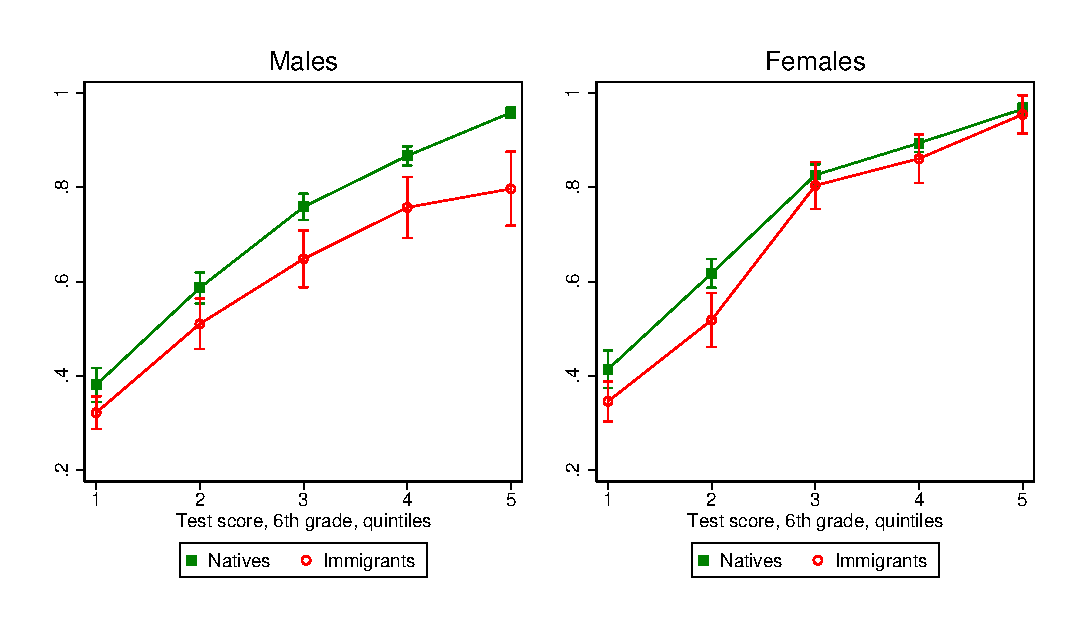
\includegraphics[scale=1]{figure_educationalchoices_f.eps}

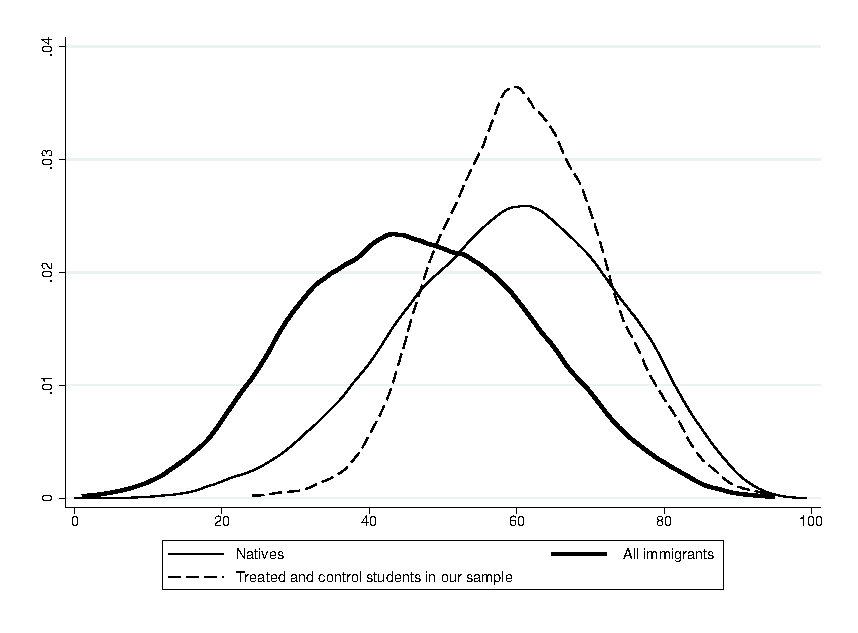
\includegraphics[scale=1]{distinvalsi6_f.eps}

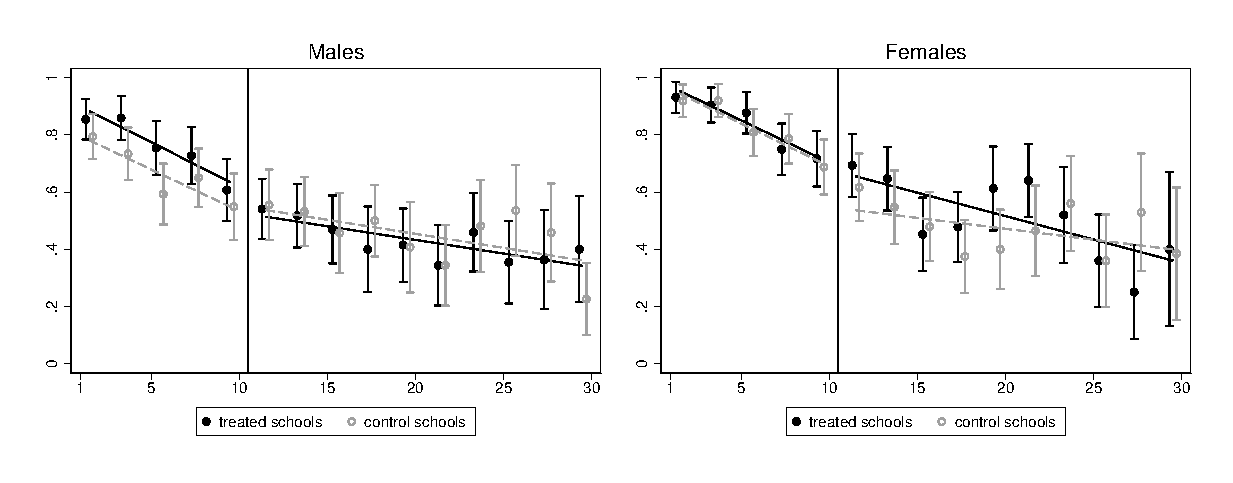
\includegraphics[scale=0.9]{rdd_top10_f.eps}

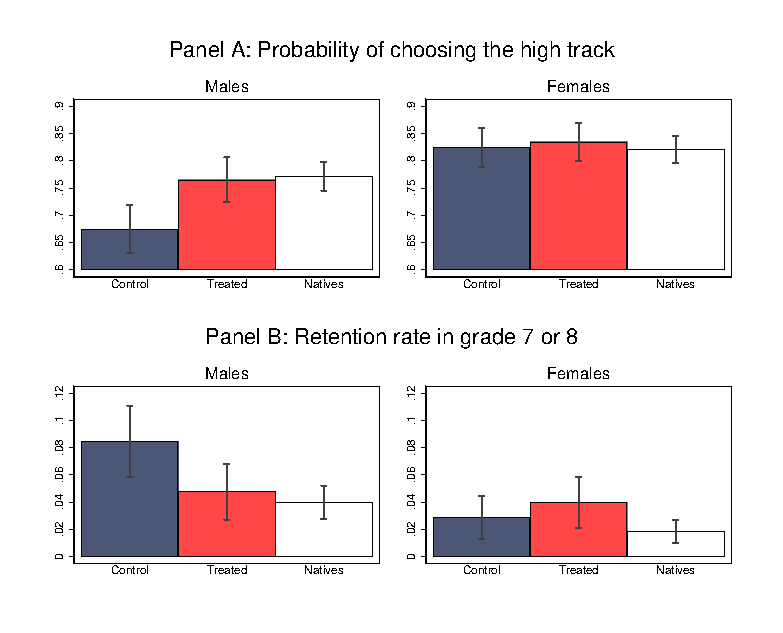
\includegraphics[scale=1.3]{figure_treatmenteffects_f.eps}

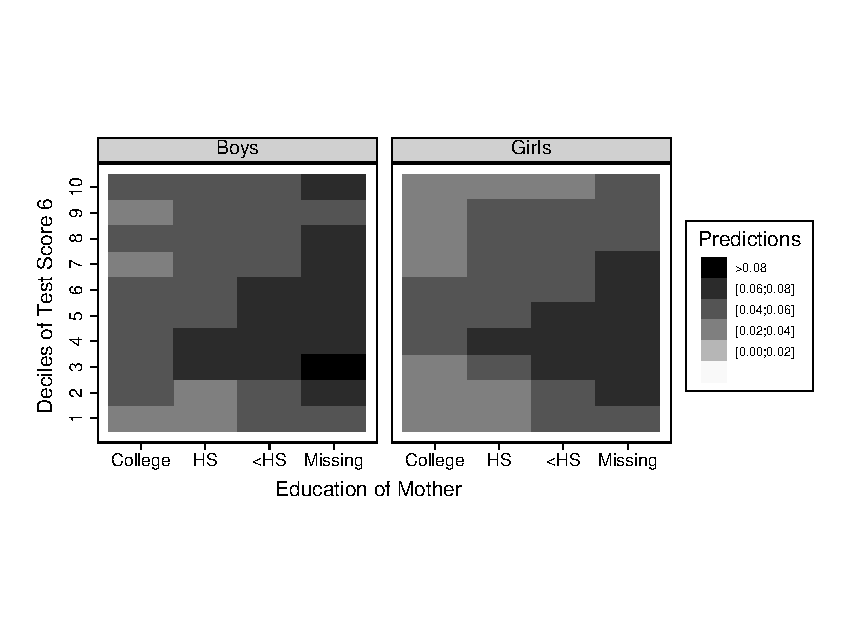
\includegraphics[scale=1.2]{Figure_heatmap1_f.eps}

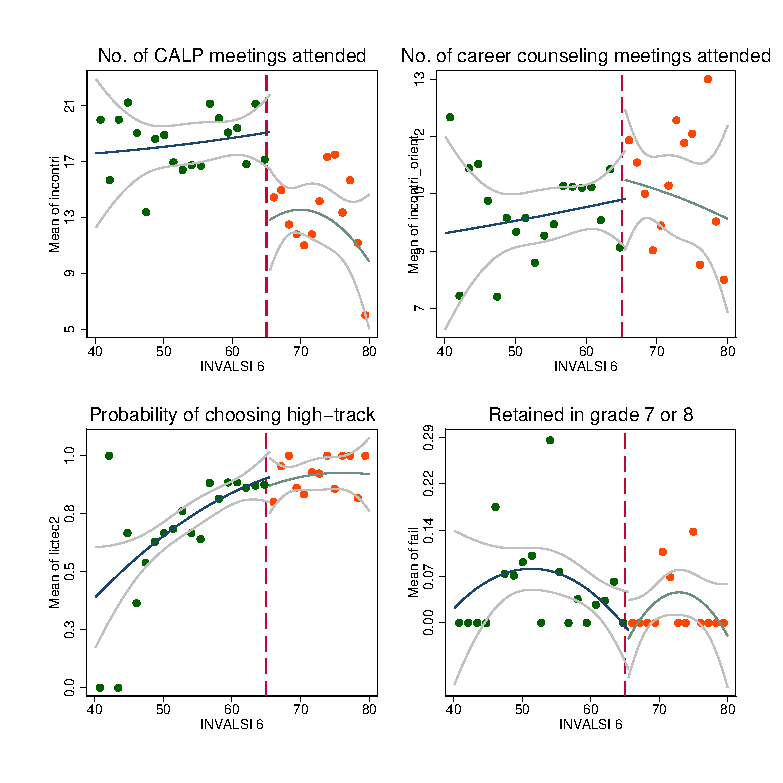
\includegraphics[scale=1.2]{figure_discontinuity_a_f.eps}

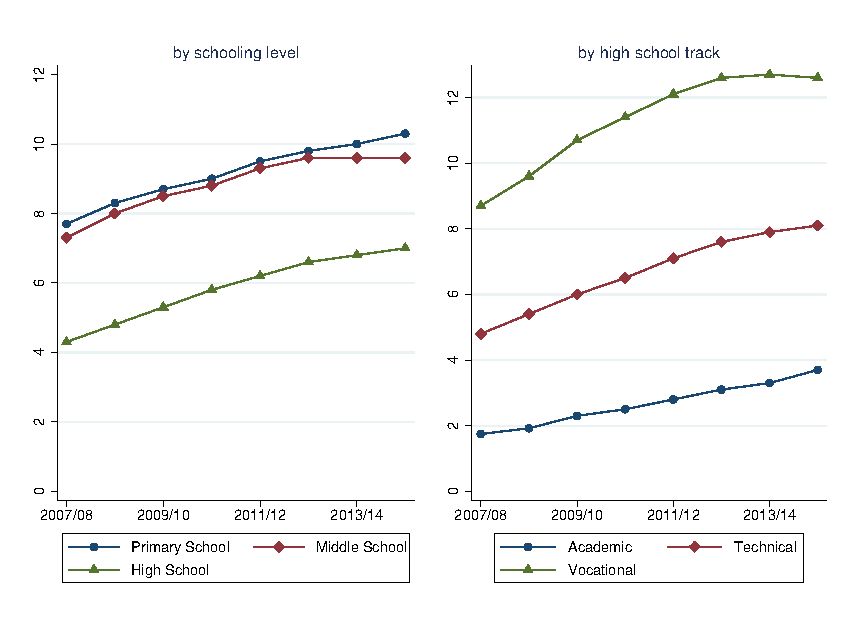
\includegraphics[scale=1.2]{immigrants_in_education_f.eps}

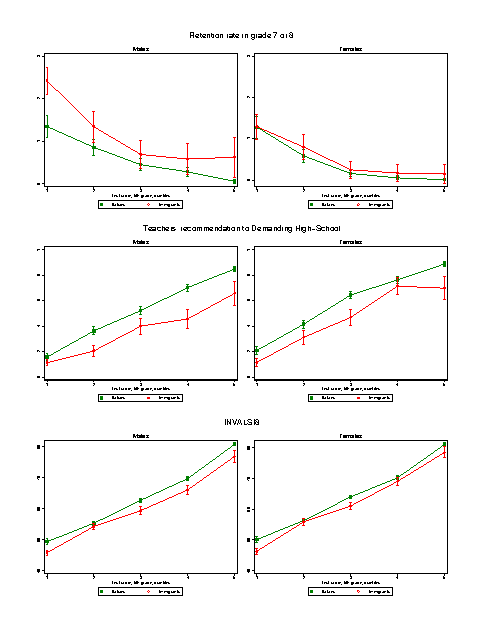
\includegraphics[scale=1.9]{Figure_segregation_other_f.eps}

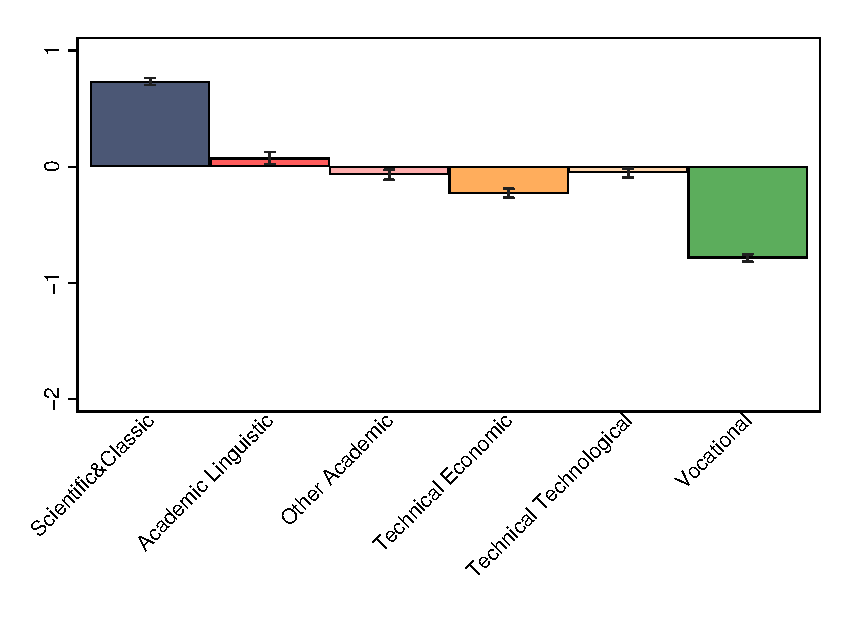
\includegraphics[scale=1.2]{Figure_choice_test_f.eps}

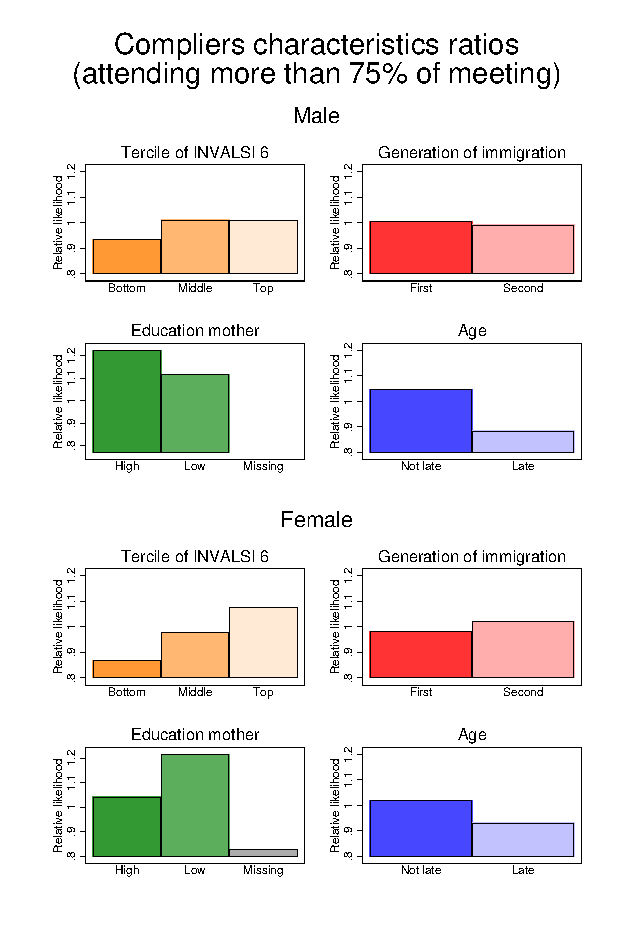
\includegraphics[scale=1.4]{Figure_compliers_f.eps}

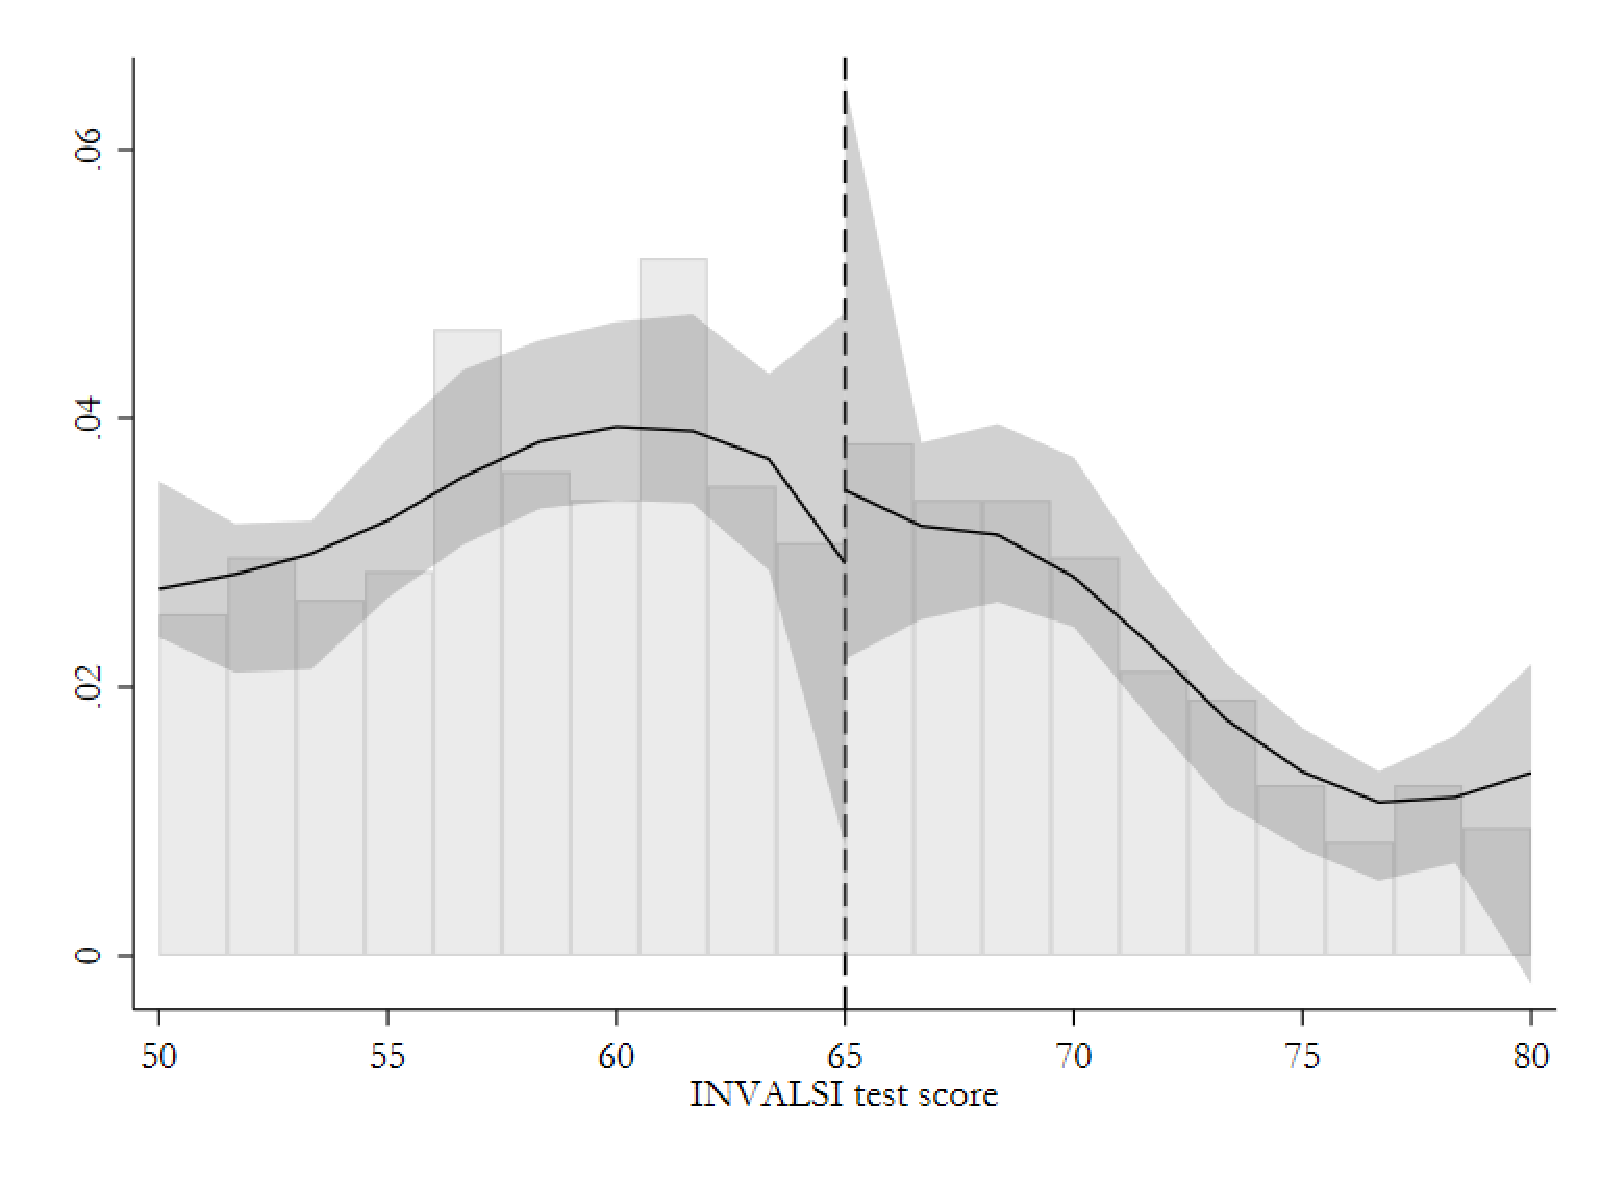
\includegraphics[scale=0.6]{mccracy_BW_f.eps}


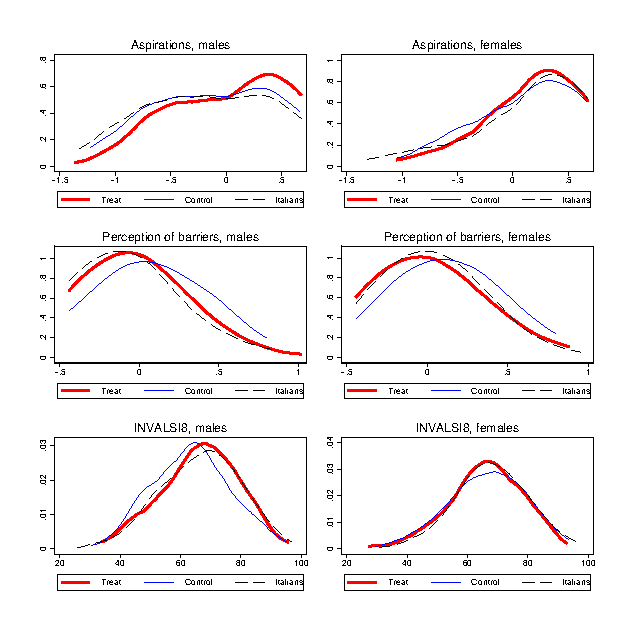
\includegraphics[scale=1.6]{figure_distributions_f.eps}

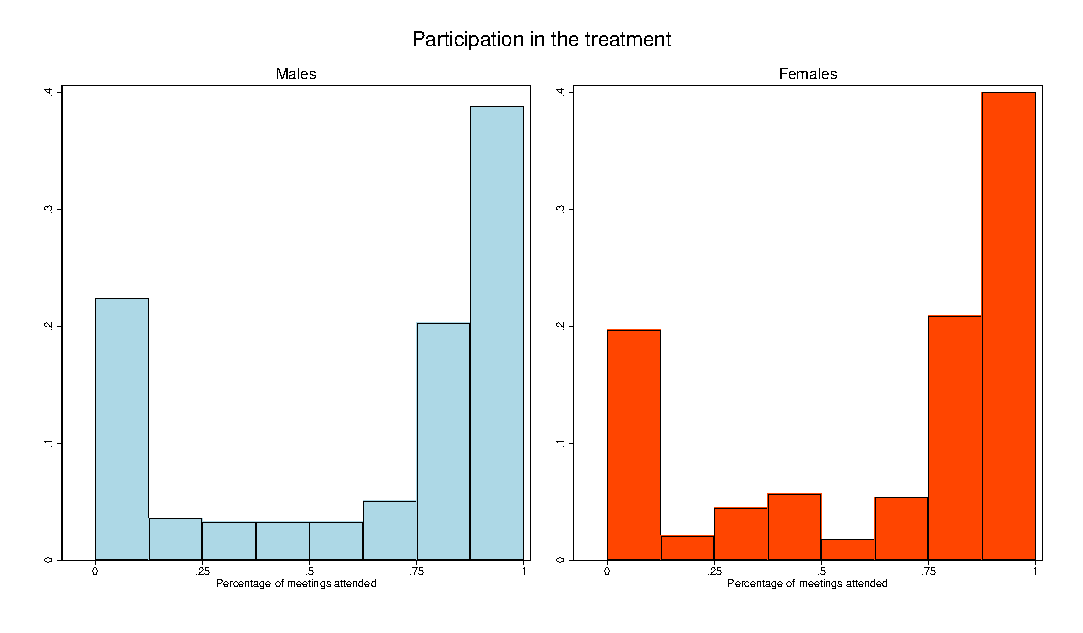
\includegraphics[scale=0.9]{compliance_f.eps}




\end{document}
